\section{Performance Evaluation}\label{section4}
In order to test the traffic differentiation capabilities of CSMA/ECA$_{\text{QoS}}$ we have used a customised version of the COST simulator~\cite{COST}, which is available via~\cite{CSMA-ECA-HEW}. If not expressed otherwise, each point in the presented figures (including Figures~\ref{fig:CAvsECA} and \ref{fig:col-CAvsECA}) is obtained from averaging fifty executions of duration equal to one hundred seconds. Further considerations:
	\begin{itemize}
		\item Unspecified parameters follow the IEEE 802.11n ($2.4$~GHz) standard.
		\item All nodes can be assumed to be in communication range with each other.
		\item Not using Request-to-Send (RTS) or Clear-to-Send (CTS) messages.
		\item Collisions are assumed to take as much channel time as successful transmissions.
	\end{itemize}

Additionally, Table~\ref{tab:mac-params} provides information about relevant PHY and MAC parameters used in the simulator.
	\begin{table}
		\centering
		\caption{PHY and MAC parameters for the simulations}
		\label{tab:mac-params}
		\begin{tabular}{|c|c|}
			\hline
			\multicolumn{2}{|c|}{{\bfseries PHY}}\\
			\hline
			{\bfseries Parameter} & {\bfseries Value}\\
			\hline
			PHY rate & 65~Mbps\\
			Empty slot & $9~\mu s$\\
			DIFS & $28~\mu s$\\
			SIFS & $10~\mu s$\\
			\hline
			\multicolumn{2}{|c|}{{\bfseries MAC}}\\
			\hline
			{\bfseries Parameter} & {\bfseries Value}\\
			\hline
			Maximum retransmission attempts & 7\\
			Packet size (Bytes) & 1024\\
			MAC queue size (Packets) & 1000\\
			\hline
		\end{tabular}
	\end{table}
	
	\begin{table}[t]
		\centering
		\caption{Updated CSMA/ECA$_{\text{QoS}}$ contention parameters for the simulations}
		\label{tab:newQoSparams}
		\begin{tabular}{|c|c|c|c|c|c|}
			\hline
			{\bfseries AC} & {\bfseries CW$_{\min}$} & {\bfseries CW$_{\max}$} & {\bfseries m} & {\bfseries lowest $B_{\text{d}}$} & {\bfseries highest $B_{\text{d}}$}\\
			\hline
			BK		       &	32				&		1024		  & 		5	&			15		        &		511\\
			BE		       &	32				&		1024		  &		5	&			15		        &		511\\
			VI		       &	16				&		512		  & 		5	&			7		        &		255\\
			VO		       &	8				&		256		  & 		5	&			3		        &		127\\
			Legacy	       &	32				&		1024		  & 		5	&			15		        &		511\\
			\hline
		\end{tabular}
	\end{table}
	
Apart from the assumptions presented above, the followings provide details about the traffic source generator, channel conditions and overall scenarios to be evaluated. Then, simulation results for achieved throughput, number of collisions and time between successful transmissions are presented.

\subsection{Simulation parameters}\label{subsect:simParams}
\subsubsection{Traffic conditions}
There are two main scenarios regarding traffic generation in a node. The \emph{saturated} traffic condition refers to a node that always has a packet for transmission in its MAC queue. On the other hand, a \emph{non-saturated} node  can also empty its MAC queue and withdraw from the channel contention. These states do not fall far from reality, for instance, a node might be in saturation while it is performing a file transfer. But if instead the node is only uploading a short file, does nothing for a period of time and then continues to perform a voice call over the network, its traffic will be considered to be non-saturated over that period of time.

In our simulator we mimic this behaviour by defining a packet arrival rate ($\Delta\text{P}$). To simulate a saturated network, for instance, we set $\Delta\text{P}$ in every node to the channel capacity. If non-saturated traffic is the goal, $\Delta\text{P}$ will be set to a value way below the system maximum aggregated throughput in order to induce periods of inactivity upon each node. After extensive tests, $\Delta\text{P}=2\text{Mbps}$ has proved to provide satisfactory results.

The performance in non-saturation for EDCA and CSMA/ECA$_{\text{QoS}}$ will be greatly dependent on the share of $\Delta\text{P}$ each AC gets, that is, the percentage of generated traffic that is going to be assigned to each AC. These shares, denoted $\Delta\text{P}_{\text{AC}}$ are distributed in the following way: $\Delta\text{P}_{\text{BK}}=0.4\Delta\text{P}$, $\Delta\text{P}_{\text{BE}}=0.3\Delta\text{P}$, $\Delta\text{P}_{\text{VI}}=0.15\Delta\text{P}$ and $\Delta\text{P}_{\text{VO}}=0.15\Delta\text{P}$. These values comply with the desired scenario.

%	\begin{table}
%		\centering
%		\caption{Shares of $\Delta\text{P}$ to each AC}
%		\label{tab:pacShares}
%		\begin{tabular}{|c|c|}
%			\hline
%			{\bfseries AC} & {\bfseries $\Delta\text{P}_{\text{AC}}$}\\
%			\hline
%			BK	&	40\%\\
%			\hline
%			BE	&	30\%\\
%			\hline
%			VI	&	15\%\\
%			\hline
%			VO	&	15\%\\
%			\hline
%		\end{tabular}
%	\end{table}
	
\subsubsection{Channel errors}
The inability to receive an ACK frame is handled as a collision, both in EDCA and CSMA/ECA$_{\text{QoS}}$. This could happen due to channel imperfections preventing the receiver from decoding the transmissions. In order to simulate the effects of channel errors over the MAC protocol, we define the likelihood of a packet not being acknowledged, $p_e$. It affects every packet independently. That is, for every packet being transmitted we draw a number from a random variable $X\sim\mathcal{U}[0,1]$, if the number drawn is lower than $p_e$ the packet will not be acknowledged. In the case of an aggregation of several packets, it is considered a failed transmission only if all packets in the aggregation are affected negatively by $p_e$. A value of $p_e=0.1$ has been selected for the simulations.

\subsubsection{Scenarios to test}
In this work we propose two main scenarios: saturation and non-saturation. The non-saturation scenario will be composed of nodes with $\Delta\text{P}=2\text{Mbps}$.

%////////////////////////////////////////////////////////////////////////////////////
%///////////////////////////////////////%Results%////////////////////////
%///////////////////////////////////////////////////////////////////////////////////

\begin{figure*}[tb]
	\centering
		\includegraphics[width=0.55\linewidth,angle = -90]{figures/multiplot-sat-perfect.eps}
		\caption{Average Aggregated Throughput and Collisions for a) EDCA, b) CSMA/ECA$_{\text{QoS}}$ and c) CSMA/ECA$_{\text{QoS}}$ in saturation with parameters from Table~\ref{tab:newQoSparams}}
		\label{fig:multiplotSat}
\end{figure*}

\begin{figure*}[tb]
	\centering
		\includegraphics[width=0.55\linewidth,angle = -90]{figures/multiplot-unsat-error-0-1.eps}
		\caption{Average Aggregated Throughput, Collisions and Time Between Successful Transmissions for a) EDCA and b) CSMA/ECA$_{\text{QoS}}$ and c) CSMA/ECA$_{\text{QoS}}$ network (without Fair Share) in non-saturation}
		\label{fig:multiplotUnsat}
\end{figure*}
	
\begin{figure*}[t]
	\centering
		\includegraphics[width=0.55\linewidth,angle = -90]{figures/multiplot-combined-unsat-error-0-1.eps}
		\caption{Average aggregated throughput, Collisions and time between successful transmissions for a) EDCA nodes and b) CSMA/ECA$_{\text{QoS}}$ nodes and c) CSMA/ECA$_{\text{QoS}}$ network (without Fair Share) nodes in a 50\%-50\% mixed non-saturated network}
		\label{fig:multiplotCombinedUnsat}
\end{figure*}

\subsection{Simulation Results}\label{sim:results}
\subsubsection{System throughput and collisions}
\begin{itemize}
\item\underline{Saturation:} Figure~\ref{fig:multiplotSat} gathers the simulation results for average aggregated throughput and collisions in a saturated network. Referring to EDCA results as Figure~\ref{fig:multiplotSat}-a,  it shows that the AC with the highest priority, AC[VO]\footnote{Starting at this point, ACs will be referred to as AC[\emph{x}], where `\emph{x}' is the abbreviation of the AC name, as in Table~\ref{tab:prioritiesMap}.}, achieves greater throughput than the others. This is a direct consequence of effective traffic differentiation in EDCA. The lower row of Figure~\ref{fig:multiplotSat} shows the total number of collisions as well as the average percentage of collisions suffered by each AC. 

Figure~\ref{fig:multiplotSat}-a also shows that AC[BK] is not able to achieve significant throughput for a high number of contenders. This is because its transmission attempts are being deferred in order to serve the high priority ACs. Furthermore, EDCA collisions show that at around 30 contenders AC[BE] also starts to get its transmission attempts deferred, easing the contention process for high priority ACs. This is the main reason of the overall throughput increase seen in Figure~\ref{fig:multiplotSat}-a at around 30 nodes.

Figure~\ref{fig:multiplotSat}-b shows the average aggregated throughput and collisions of a saturated CSMA/ECA$_{\text{QoS}}$ network using the default contention parameters (see Table~\ref{tab:ecaQosParams}). These settings do not allow the construction of collision-free schedules for many contenders. This is evidenced by the high number of collisions at around 20 contenders. Moreover, the figure shows CSMA/ECA$_{\text{QoS}}$ throughput decreasing faster than EDCA.

To allow the construction of collision-free schedules, the contention parameters for CSMA/ECA$_{\text{QoS}}$ are modified to the ones shown in Table~\ref{tab:newQoSparams}. These new parameters allow the construction of larger collision-free schedules, therefore allow collision-free operation with a larger number of contenders. Figure~\ref{fig:multiplotSat}-c provides throughput and collisions results with these new contention parameters. The figure shows higher throughput for a wider number of contenders, as opposed to EDCA, where it decreases rapidly as contenders join the network. Further, collisions start to increase at around 32 contenders, which is the maximum number of saturated collision-free contenders supported with the updated contention parameters. It is relevant to highlight that unlike EDCA, CSMA/ECA$_{\text{QoS}}$ is able to accommodate transmissions for every AC when there is a high number of contenders (e.g.: $N\geq 40$). In the same manner, Figure~\ref{fig:multiplotSat}-c also shows a clear reduction in the number of collisions when using CSMA/ECA$_{\text{QoS}}$.

The updated parameters for CSMA/ECA$_{\text{QoS}}$ (Table~\ref{tab:newQoSparams}) make a tradeoff between throughput and aggressiveness. Allowing CSMA/ECA$_{\text{QoS}}$'s deterministic backoffs to grow past EDCA's default parameters increases the time between successful transmissions, but also avoids starving low priority ACs and provide a greater overall throughput (due to a reduction in the number of collisions and the aggregation performed by Fair Share).

\item\underline{Non-Saturation:}

In the non-saturation scenario, nodes in the network have $\Delta\text{P}=2$Mbps. Moreover, the shares of $\Delta\text{P}$ assigned to each AC are defined in Section~\ref{subsect:simParams}. Results are derived from simulations performed with $p_e=0.1$.

	\begin{table}[t]
		\centering
		\caption{Saturation points in non-saturation scenarios ($N$)}
		\label{tab:satPoints}
		\begin{tabular}{|c|c|c|c|c|}
			\hline
			{\bfseries Protocol} 				& {\bfseries BK} & {\bfseries BE} & {\bfseries VI} & {\bfseries VO}\\
			\hline
			EDCA						&	10		&	16		&		22	&	22\\	
			\hline
			CSMA/ECA${\text{QoS}}$		&	14		&	16		&		36	&	50\\
			\hline
			CSMA/ECA${\text{QoS}}$ w/o FS	&	10		&	16		&		28	&	28\\
			\hline
		\end{tabular}
	\end{table}

Figure~\ref{fig:multiplotUnsat} shows the (from top to bottom row) average aggregated throughput, collisions and time between successful transmissions for (from left to right column) a) EDCA, b) CSMA/ECA$_{\text{QoS}}$ and c) CSMA/ECA$_{\text{QoS}}$ without Fair Share. In Figure~\ref{fig:multiplotUnsat}-a, EDCA throughput keeps increasing up until one of its ACs reaches saturation due to starvation. This is the case of AC[BK] at around $N=10$. It is only at around $N=24$ where the rest of ACs get completely saturated, and both figures start to resemble the ones presented in the saturation case.

\begin{figure}[t!]
	\centering
		\includegraphics[width=1.1\linewidth,angle = -90]{figures/legacyEvolution.eps}
		\caption{Throughput for a mixed network setup with 20 contenders in non-saturation: a) Overall throughput, b) Throughput of AC[BK], c) Throughput of AC[VO]}
		\label{fig:legacyEvolution}
\end{figure}

In Figure~\ref{fig:multiplotUnsat}-b at $N\leq 14$, contenders join and withdraw from the contention more frequently. This causes a disruption of any existing collision-free schedule, which is represented by the increase in collisions at $N=14$. Once ACs get saturated, more periods of collision-free operation are achieved, accounting for the subsequent reduction in the total number of collisions.

Even-though $p_e$ induces retransmissions that degrade the performance, throughput gains and collision reductions with CSMA/ECA$_{\text{QoS}}$ are maintained. This is mainly due to the level of stickiness used and the additional increase provided by the Schedule Reset mechanism (see Section~\ref{scheduleReset}).


%	\begin{figure}[tb]
%	\centering
%		\includegraphics[width=0.7\linewidth,angle = -90]{figures/diffThroughputPlot-unsat-error-0-1.eps}
%		\caption{CSMA/ECA$_{\text{QoS}}$ average aggregated throughput in non-saturated conditions, $p_e=0.1$, normalised to EDCA's}
%		\label{fig:diffThroughput-unsat-error-0.1}
%	\end{figure}
%
%	\begin{figure}[tb]
%	\centering
%		\includegraphics[width=0.7\linewidth,angle = -90]{figures/diffCollisionsPlot-unsat-error-0-1.eps}
%		\caption{CSMA/ECA$_{\text{QoS}}$ collisions in non-saturated conditions, $p_e=0.1$, normalised to EDCA's}
%		\label{fig:diffCollisions-unsat-error-0.1}
%	\end{figure}

\end{itemize}

\subsubsection{Average time between successful transmissions}
This metric refers to the average time between two consecutive successful transmissions of each AC. Figure~\ref{fig:multiplotUnsat}-a shows that despite preventing transmissions from low priority ACs, AC[VO] and AC[VI] maintain a fairly low metric. This is specially relevant for time sensitive applications, like voice or video calls. Nevertheless, it implies that while high priority ACs are saturated, there is no effective throughput for other kind of traffic.

On the other hand, as shown in Figure~\ref{fig:multiplotUnsat}-b, CSMA/ECA$_{\text{QoS}}$ takes more time between successful transmissions. This is partly because of the packet aggregation performed by Fair Share, which make transmissions longer. Furthermore, as low priority ACs are also transmitting, these also contribute to the increase in the time between successful transmissions. 

Although EDCA keeps the time between successful transmissions very low, it does so by almost preventing low priority ACs from accessing the channel. If Fair Share is deactivated in CSMA/ECA$_{\text{QoS}}$, the overall throughput might get negatively affected (no aggregation is performed), but the time between successful transmissions will be reduced, as shown in Figure~\ref{fig:multiplotUnsat}-c.

Table~\ref{tab:satPoints} shows the saturation points for each protocol. That is, the number of nodes at which the network gets saturated. As it can be seen in the table, CSMA/ECA${\text{QoS}}$ saturates at higher number of contenders, providing higher throughput for a wider number of users than EDCA.

\subsubsection{Coexistence with EDCA}
	
The followings are extracted from simulations performed with a network setup composed of 50\% EDCA nodes and 50\% CSMA/ECA$_{\text{QoS}}$ in non-saturation and $p_e=0.1$. Figure~\ref{fig:multiplotCombinedUnsat} shows (from first to last row) average aggregated throughput, collisions and average time between successful transmissions for each group of nodes (from left to right column): a) EDCA nodes, b)CSMA/ECA$_{\text{QoS}}$ nodes and an additional test with c) CSMA/ECA$_{\text{QoS}}$ without Fair Share (w/o FS) nodes. The Fair Share mechanism is deactivated in order to reduce the time between successful transmissions.

%Figure~\ref{fig:throughputCombined-vs-EDCA} shows the aggregated throughput gain when compared against a 100\% EDCA network with the same traffic and error parameters. The collision-free periods experienced by the CSMA/ECA$_{\text{QoS}}$ nodes account for the throughput increase seen in the figure. Furthermore, as Figure~\ref{fig:collisionsCombined-vs-EDCA} shows, the overall collisions are reduced for the same reason.

%THINK THIS. FIND AN EXPLANATION!!!!!!!! 
%hint 1: the time between successful transmissions of CSMA/ECA stations in this mixed network, is lower than EDCA (for high number of nodes). Further, if collisions are high, this means that the contention parameters of EDCA is not able to support many contenders, killing EDCA stations's throughput.
%hint 2: COLLISIONS ARE ALMOST 99% for the only two high priority ACs (high number of nodes).
%hint 3: at lower number of nodes: the high time between successful transmissions is due to CSMA/ECA nodes being able to perform transmissions for all its ACs, while EDCA stations defer more aggressively in order to serve high priority ACs.

%FINAL HINT: At low number of nodes, EDCA has lower delay and higher throughput becasue it is much more aggressive in the traffic differentiation, prioritising ACs and being very aggressive with its contention parameters. In the mixed network, CSMA/ECAqos nodes elevate the average delay too much due to its less aggresive contention. At high number of nodes the mixed network goes worst than EDCA, but this is mostly due to EDCA nodes, which elevate the average collisions, delay and decrement the overall throughput.

Even-though there are periods of collision-free operation, which are evidenced by the higher throughput experienced by CSMA/ECA$_{\text{QoS}}$ nodes in Figure~\ref{fig:multiplotCombinedUnsat}-b, Figure~\ref{fig:multiplotCombinedUnsat}-c shows that the time between successful transmissions can be further reduced by not using FS. Deactivating Fair Share causes a degradation in the overall throughput and an increase in the number of collisions, mostly due to reaching the saturation point faster (at lower $N$). Nevertheless, Figure~\ref{fig:multiplotCombinedUnsat}-c shows that CSMA/ECA$_{\text{QoS}}$ w/o FS nodes still experience higher throughput, lower collisions and similar time between successful transmissions than EDCA nodes, both in Figure~\ref{fig:multiplotCombinedUnsat}-a and in a EDCA-only network, shown in Figure~\ref{fig:multiplotUnsat}-a.

%it still offers higher throughput  a metric of time between successful transmissions similar to

%Even-though there are periods of collision-free operation, Fair Share increases the average time between successful transmissions of high priority ACs. This is shown in Figure~\ref{fig:multiplotUnsat}-b, where said metric for the mixed network is compared against a EDCA-only network. Repeating the same test with Fair Share deactivated in CSMA/ECA$_{\text{QoS}}$ yields the results shown in Figure~\ref{fig:timeCombined-vs-EDCA-hystOnly}.

EDCA takes a much more aggressive approach towards providing traffic differentiation, mostly due to its tight contention parameters and AIFS. On the other hand, even at low number of contenders EDCA's tight contention parameters provoke an increase in the number of collisions. Furthermore, it starves low priority ACs (like BK and BE); increasing the delay consequently (see Figure~\ref{fig:multiplotCombinedUnsat}-a).

Figure~\ref{fig:legacyEvolution} shows the a) overall, b) AC[BK], and c) AC[VO] throughput for a non-saturated mixed network with $p_e=0.1$ and 20 contenders as the percentage of EDCA nodes increases from 0 to 100\%. Figure~\ref{fig:legacyEvolution}-a shows that both protocols' aggregated throughput decreases as a consequence of the coexistence. Nevertheless, CSMA/ECA$_{\text{QoS}}$ nodes aggregated throughput is higher for a larger proportion of EDCA nodes than the other way around. This is mainly because CSMA/ECA$_{\text{QoS}}$ nodes do not starve low priority ACs.

AC[BK] for EDCA nodes in Figure~\ref{fig:legacyEvolution}-b shows little variation. As seen in Figure~\ref{fig:multiplotUnsat}-a, at this number of contenders ($N=20$) AC[BK] has almost no throughput due to starvation by EDCA. On the other hand, for CSMA/ECA$_{\text{QoS}}$ this low priority AC shows higher throughput even for high percentages of EDCA nodes ($<90\%$).

Figure~\ref{fig:legacyEvolution}-c, showing AC[VO]'s throughput, is consistent with Figure~\ref{fig:legacyEvolution}-a, that is, it is possible to observe a throughput degradation due to the coexistence in both protocol. Nevertheless, AC[VI] throughput degrades almost at the same rate for both protocols (same slope $\pm 0.6$).

